\begin{frame}{‌تحلیل تجمعی}
\begin{itemize}\itemr
\item[-]
یک نوع دیگر تحلیل الگوریتم‌ها تحلیل تجمعی
\fn{1}{aggregate analysis}
 است.
\item[-]
در تحلیل تجمعی
، نشان می‌دهیم دنباله‌ای از n عملیات در بدترین حالت به زمان
\m{T(n)}
نیاز دارد.
\item[-]
بنابراین در بدترین حالت، هزینهٔ متوسط یا هزینهٔ سرشکن
\fn{2}{amortize}
، به ازای هریک از عملیات برابراست با
\m{T(n)/n} .
\item[-]
هزینهٔ به دست آمده، هزینهٔ متوسطی است که به ازای هر یک از عملیات نیاز است حتی اگر برخی از عملیات به زمان کمتری نیاز داشته باشند.
\end{itemize}
\end{frame}

\iffalse
\begin{frame}{‌تحلیل تجمعی}
\begin{itemize}\itemr
\item[-]
می‌خواهیم عملیات مربوط به یک پشته را با استفاده از تحلیل تجمعی تحلیل کنیم.
\item[-]
تابع
\m{Push(S,x)}
شیء 
\m{x}
 را در پشته 
\m{S}
  قرار می‌دهد و تابع
\m{Pop(S)}
یک شیء از پشته استخراج می‌کند. فراخوانی
\m{Pop}
با پشتهٔ خالی منجر به خطا می‌شود.
\end{itemize}
\end{frame}


\begin{frame}{‌تحلیل تجمعی}
\begin{itemize}\itemr
\item[-]
هزینهٔ هریک از عملیات پشته
\m{O(1)}
است. فرض کنیم هزینهٔ انجام این عمل به میزان ۱ واحد زمان باشد. مجموع هزینه‌های دنباله‌ای از n عملیات
\m{Push}
و
\m{Pop}
برابراست با n و زمان اجرای n عملیات
\m{O(n)}
است.
\item[-]
حال یک عملگر جدید به نام
\m{Multipop(S,k)}
می‌افزاییم که با استفاده از آن k شیء از روی پشته S برداشته می‌شود و در صورتی که تعداد اشیای درون پشته کمتر از k باشد، همهٔ اشیای پشته حذف می‌شوند.
\end{itemize}
\end{frame}


\begin{frame}{‌تحلیل تجمعی}
\begin{itemize}\itemr
\item[-]
الگوریتم تابع
\m{Multipop}
به صورت زیر است.
\begin{algorithm}[H]\alglr
  \caption{Multipop} 
  \begin{algorithmic}[1]
   \Func{Multipop}{S, k}
        \While{not Stack-Empty(S) and k > 0}
        		\State Pop(S)
        		\State k = k - 1
         \EndWhile
  \end{algorithmic}
  \label{alg:merge}
\end{algorithm}
\end{itemize}
\end{frame}


\begin{frame}{‌تحلیل تجمعی}
\begin{itemize}\itemr
\item[-]
حال می‌خواهیم زمان اجرای
\m{Multipop(S,k)}
را بر روی یک پشته با s شیء محاسبه کنیم.
\item[-]
زمان اجرای این تابع وابسته به زمان اجرای
\m{Pop}
است. تعداد تکرارهای حلقه در این الگوریتم برابراست با
\m{min\{s,k\}}
و چون
\m{Pop}
به زمان ثابت برای اجرا نیاز دارد، تعداد تکرارهای کل برابر می‌شود با
\m{min\{s,k\}}.
\end{itemize}
\end{frame}


\begin{frame}{‌تحلیل تجمعی}
\begin{itemize}\itemr
\item[-]
حال دنباله‌ای از n عملیات
\m{Push}
و
\m{Pop}
و
\m{Multipop}
را در نظر بگیرید. فرض کنید یک پشتهٔ خالی داریم و می‌خواهیم این عملیات را بر روی پشته انجام دهیم.
\item[-]
اگر بخواهیم زمان اجرای کل عملیات را تحلیل کنیم، می توانیم بگوییم در بدترین حالت n عملیات
\m{Multipop}
داریم که هرکدام در زمان
\m{O(n)}
انجام می‌شوند و بنابراین در مجموع زمان اجرا
\m{O(n^2)}
است.
\item[-]
اما اگر بخواهیم با تحلیل تجمعی زمان اجرا این عملیات را تحلیل کنیم، می‌گوییم عملیات
\m{Multipop}
بدون انجام عملیات
\m{Push}
نمی‌تواند انجام بگیرد، بنابراین در بدترین حالت در مجموع به
\m{O(n)}
زمان نیاز داریم و اگر این زمان را به تعداد عملیات تقسیم کنیم، زمان میانگین به ازای هر یک از عملیات برابراست با
\m{O(n)/n = O(1)}
\end{itemize}
\end{frame}
\fi

\begin{frame}{‌تحلیل تجمعی}
\begin{itemize}\itemr
\item[-]
یک مثال از تحلیل تجمعی را بررسی می‌کنیم.
\item[-]
یک شمارندهٔ دودویی k بیتی را در نظر بگیرید که از صفر شروع به شمارش می‌کند.
\item[-]
فرض کنید برای شمارنده از آرایهٔ
\m{A[0 : k-1]}
استفاده کنیم. توسط آرایهٔ A عدد x نشان داده می‌شود به طوری‌که
\begin{align*}
\m{x = \sum_{i = 0}^{k-1} A[i] \times 2^i}
\end{align*}
\end{itemize}
\end{frame}


\begin{frame}{‌تحلیل تجمعی}
\begin{itemize}\itemr
\item[-]
می‌خواهیم الگوریتمی بنویسیم که مقدار این شمارندهٔ k بیتی را یک واحد افزایش دهد.
الگوریتم زیر نحوهٔ اجرای این شمارنده را نشان می‌دهد.
\begin{algorithm}[H]\alglr
  \caption{Increment} 
  \begin{algorithmic}[1]
   \Func{Increment}{A, k}
    \State i = 0
    \While{i < k and A[i] == 1}
    		\State A[i] = 0
    		\State i = i + 1
    \EndWhile
    \If{i < k}
    		\State A[i] = 1
    \EndIf                  
  \end{algorithmic}
  \label{alg:merge}
\end{algorithm}
\end{itemize}
\end{frame}


\begin{frame}{‌تحلیل تجمعی}
\begin{itemize}\itemr
\item[-]
شکل زیر مقدار آرایهٔ A را به ازای هر یک از اعداد شمارنده نشان می‌دهد. هزینهٔ افزایش شمارنده (تعداد تکرارهای حلقه در الگوریتم شمارش) به ازای هر شمارش و همچنین به طور تجمعی در سمت راست نشان داده شده است.
\begin{figure}
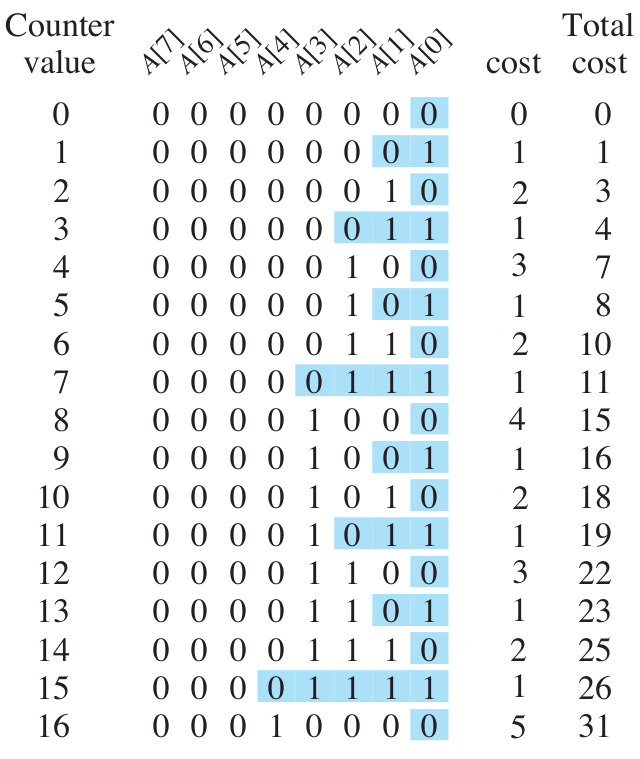
\includegraphics[width=0.3\textwidth]{figs/chap02/counter-example2}
\end{figure}
\end{itemize}
\end{frame}


\begin{frame}{‌تحلیل تجمعی}
\begin{itemize}\itemr
\item[-]
فرض کنید می‌خواهیم n واحد به شمارنده بیافزاییم.
\item[-]
در اینجا با یک تحلیل ساده می‌توانیم زمان اجرا را به دست آوریم.
\item[-]
یک بار اجرای الگوریتم در بدترین حالت در زمان
\m{O(k)}
اجرا می‌شود.
\item[-]
بنابراین دنباله‌ای از n عملیات به زمان
\m{O(nk)}
در بدترین حالت نیاز دارد.
\end{itemize}
\end{frame}


\begin{frame}{‌تحلیل تجمعی}
\begin{itemize}\itemr
\item[-]
اما اگر بخواهیم دقیق‌تر به طور تجمعی این الگوریتم را برای n عملیات تحلیل کنیم، می‌بینیم
\m{A[0]}
به ازای هر واحد افزایش یک بار تغییر می‌کند،
\m{A[1]}
به ازای هر دو واحد افزایش شمارنده یک بار تغییر می‌کند،
\m{A[2]}
به ازای هر چهار واحد افزایش شمارنده یک بار تغییر می‌کند، الی آخر.
\item[-]
بنابراین پس از n واحد افزایش شمارنده،
\m{A[0]}
تعداد n بار،
\m{A[1]}
تعداد
\m{\lfloor n/2 \rfloor}
بار، و
\m{A[2]}
تعداد
\m{\lfloor n/4 \rfloor}
بار ، و به طور کل
\m{A[i]}
تعداد
\m{\lfloor n/2^i \rfloor}
تغییر می‌کند.
\item[-]
بنابراین در مجموع برای n واحد افزایش شمارنده k بیتی، تعداد تغییرات بیت‌ها به صورت زیر محاسبه می‌شوند.
\begin{align*}
\m{\sum_{i = 0}^{k - 1} \lfloor \frac{n}{2^i} \rfloor < n \sum_{i = 0}^{\infty} \frac{1}{2^i} = 2n}
\end{align*}
\item[-]
بنابراین در مجموع این شمارنده پس از n واحد افزایش در زمان
\m{O(n)}
اجرا می‌شود و میانگین زمان اجرا و هزینه سرشکن به ازای یک واحد افزایش برابراست با
\m{O(n)/n = O(1)}.
\end{itemize}
\end{frame}